\documentclass{article}
\title{Project 2\\ Getting Shit Done and Doin' Work}
\author{Nat Hawkins, Victor Ramirez, Mike Roosa, Pranjal "Danger" Tiwari}
\date{27 February, 2017}

\usepackage{relsize,makeidx,color,setspace,amsmath,amsfonts,amssymb}
\usepackage[table]{xcolor}
\usepackage{bm,ltablex,microtype}
\usepackage{placeins}
\usepackage{listings}
\usepackage[top = 1in, bottom = 1in, right = 1in, left = 1in]{geometry}
\usepackage[pdftex]{graphicx}
\usepackage{epstopdf}
\usepackage{inputenc}
\usepackage{url}
\usepackage{blindtext}
\usepackage{MnSymbol,wasysym}
\usepackage[final]{pdfpages}

\begin{document}
\maketitle
\noindent
\begin{abstract}
	The goal of this project is to explore a model of quantum dots. We will be investigating the behavior of two electron in a 3-D simple harmonic potential while comparing the models with and without the particles interacting. To do this we will be solving the Schrödinger equation using the Jacobi method. What we found is that with our Jacobi eigensolver, one of the many issues surrounding it is that we do not know the maximum number of iterations needing to be performed on the matrix in question in order to get the eigenvalues. This lead to some issues in our attempts at writing the program for the eigensolver. We were able to calculate the eigenvalues for a square symmetric matrix that agree with the eigenvalues of standard python library solvers (i.e. numpy.linalg.eig). The eigensolver was also used to compute eigenvalues for a specific value of frequency, $\omega$, which we then compared to the analytic results. Our numerical values were within 0.5\% of the analytic value.
	
\end{abstract}

\section{Introduction}
Finding the eigenvalues of a matrix can give information on properties of a system, such as energies or spin. These properties can be useful to know when experiments are performed. Since we can predict the Hamiltonian of a system using the Shr$\ddot{o}$dinger equation. If we have a system with many particles, it is impractical to do so by hand, which is where computing eigenvalues from a matrix using computers becomes useful. Doing so will require a code that can find eigenvalues from a matrix, which is what the present work attempts to create.

\subsection{Mathematical Motivation}

The aim of this project is to solve Schroedinger's equation for two
electrons in a three-dimensional harmonic oscillator well with and
without a repulsive Coulomb interaction.  We aimed to solve this
equation by reformulating it in a discretized form as an eigenvalue
equation to be solved with Jacobi's method. 

Electrons confined in small areas in semiconductors, so-called quantum
dots, form a hot research area in modern solid-state physics, with
applications spanning from such diverse fields as quantum
nano-medicine to the contruction of quantum gates. 

Here we will assume that these electrons move in a three-dimensional harmonic
oscillator potential (they are confined by for example quadrupole fields)
and repel  each other via the static Coulomb interaction.  
We assume spherical symmetry.  

We are first interested in the solution of the radial part of Schroedinger's equation for one electron. This equation reads

\begin{equation*}
  -\frac{\hbar^2}{2 m} \left ( \frac{1}{r^2} \frac{d}{dr} r^2
  \frac{d}{dr} - \frac{l (l + 1)}{r^2} \right )R(r) 
     + V(r) R(r) = E R(r).
\end{equation*}
In our case $V(r)$ is the harmonic oscillator potential $(1/2)kr^2$ with
$k=m\omega^2$ and $E$ is
the energy of the harmonic oscillator in three dimensions.
The oscillator frequency is $\omega$ and the energies are

\begin{equation*}
E_{nl}=  \hbar \omega \left(2n+l+\frac{3}{2}\right),
\end{equation*}
with $n=0,1,2,\dots$ and $l=0,1,2,\dots$.

Since we have made a transformation to spherical coordinates it means that 
$r\in [0,\infty)$.  
The quantum number
$l$ is the orbital momentum of the electron.  
% 
Then we substitute $R(r) = (1/r) u(r)$ and obtain
% 

\begin{equation*}
  -\frac{\hbar^2}{2 m} \frac{d^2}{dr^2} u(r) 
       + \left ( V(r) + \frac{l (l + 1)}{r^2}\frac{\hbar^2}{2 m}
                                    \right ) u(r)  = E u(r) .
\end{equation*}
% 
The boundary conditions are $u(0)=0$ and $u(\infty)=0$.

We introduce a dimensionless variable $\rho = (1/\alpha) r$
where $\alpha$ is a constant with dimension length and get
% 

\begin{equation*}
  -\frac{\hbar^2}{2 m \alpha^2} \frac{d^2}{d\rho^2} u(\rho) 
       + \left ( V(\rho) + \frac{l (l + 1)}{\rho^2}
         \frac{\hbar^2}{2 m\alpha^2} \right ) u(\rho)  = E u(\rho) .
\end{equation*}
% 
We will set in this project $l=0$.
Inserting $V(\rho) = (1/2) k \alpha^2\rho^2$ we end up with

\begin{equation*}
  -\frac{\hbar^2}{2 m \alpha^2} \frac{d^2}{d\rho^2} u(\rho) 
       + \frac{k}{2} \alpha^2\rho^2u(\rho)  = E u(\rho) .
\end{equation*}
We multiply thereafter with $2m\alpha^2/\hbar^2$ on both sides and obtain

\begin{equation*}
  -\frac{d^2}{d\rho^2} u(\rho) 
       + \frac{mk}{\hbar^2} \alpha^4\rho^2u(\rho)  = \frac{2m\alpha^2}{\hbar^2}E u(\rho) .
\end{equation*}
The constant $\alpha$ can now be fixed
so that

\begin{equation*}
\frac{mk}{\hbar^2} \alpha^4 = 1,
\end{equation*}
or

\begin{equation*}
\alpha = \left(\frac{\hbar^2}{mk}\right)^{1/4}.
\end{equation*}
Defining

\begin{equation*}
\lambda = \frac{2m\alpha^2}{\hbar^2}E,
\end{equation*}
we can rewrite Schroedinger's equation as

\begin{equation*}
  -\frac{d^2}{d\rho^2} u(\rho) + \rho^2u(\rho)  = \lambda u(\rho) .
\end{equation*}
This is the first equation to solve numerically. In three dimensions 
the eigenvalues for $l=0$ are 
$\lambda_0=3,\lambda_1=7,\lambda_2=11,\dots .$

We use the by now standard
expression for the second derivative of a function $u$
\begin{equation}
    u''=\frac{u(\rho+h) -2u(\rho) +u(\rho-h)}{h^2} +O(h^2),
    \label{eq:diffoperation}
\end{equation}
where $h$ is our step.
Next we define minimum and maximum values for the variable $\rho$,
$\rho_{\mathrm{min}}=0$  and $\rho_{\mathrm{max}}$, respectively.
You need to check your results for the energies against different values
$\rho_{\mathrm{max}}$, since we cannot set
$\rho_{\mathrm{max}}=\infty$. 

With a given number of mesh points, $N$, we 
define the step length $h$ as, with $\rho_{\mathrm{min}}=\rho_0$  and $\rho_{\mathrm{max}}=\rho_N$,

\begin{equation*}
  h=\frac{\rho_N-\rho_0 }{N}.
\end{equation*}
The value of $\rho$ at a point $i$ is then 
\[
    \rho_i= \rho_0 + ih \hspace{1cm} i=1,2,\dots , N.
\]
We can rewrite the Schroedinger equation for a value $\rho_i$ as

\[
-\frac{u(\rho_i+h) -2u(\rho_i) +u(\rho_i-h)}{h^2}+\rho_i^2u(\rho_i)  = \lambda u(\rho_i),
\]
or in  a more compact way

\[
-\frac{u_{i+1} -2u_i +u_{i-1}}{h^2}+\rho_i^2u_i=-\frac{u_{i+1} -2u_i +u_{i-1} }{h^2}+V_iu_i  = \lambda u_i,
\]
where $V_i=\rho_i^2$ is the harmonic oscillator potential.

We define first the diagonal matrix element
\begin{equation*}
   d_i=\frac{2}{h^2}+V_i,
\end{equation*}
and the non-diagonal matrix element
\begin{equation*}
   e_i=-\frac{1}{h^2}.
\end{equation*}
In this case the non-diagonal matrix elements are given by a mere constant.
\emph{All non-diagonal matrix elements are equal}.
With these definitions the Schroedinger equation takes the following form

\begin{equation*}
d_iu_i+e_{i-1}u_{i-1}+e_{i+1}u_{i+1}  = \lambda u_i,
\end{equation*}
where $u_i$ is unknown. We can write the 
latter equation as a matrix eigenvalue problem
\begin{equation}
    \begin{bmatrix}d_0 & e_0 & 0   & 0    & \dots  &0     & 0 \\
                                e_1 & d_1 & e_1 & 0    & \dots  &0     &0 \\
                                0   & e_2 & d_2 & e_2  &0       &\dots & 0\\
                                \dots  & \dots & \dots & \dots  &\dots      &\dots & \dots\\
                                0   & \dots & \dots & \dots  &\dots  e_{N-1}     &d_{N-1} & e_{N-1}\\
                                0   & \dots & \dots & \dots  &\dots       &e_{N} & d_{N}
             \end{bmatrix}  \begin{bmatrix} u_{0} \\
                                                              u_{1} \\
                                                              \dots\\ \dots\\ \dots\\
                                                              u_{N}
             \end{bmatrix}=\lambda \begin{bmatrix} u_{0} \\
                                                              u_{1} \\
                                                              \dots\\ \dots\\ \dots\\
                                                              u_{N}
             \end{bmatrix}.  
      \label{eq:sematrix}
\end{equation}
Since the values of $u$ at the two endpoints are known via the boundary conditions, we can skip the rows and columns that involve these values. Inserting the values for $d_i$ and $e_i$ we have the a matrix form we can now use in Jacobi's Algorithm to solve for the energies. \cite{mortengithub}
The Hamiltonians that we will be concerned with will be in the form of a tridiagonal matrix and tridiagonal matrices are simple to get eigenvalues from, but if the matrix were 100x100, it would be too much to compute by hand. Therefore, the discretized method we will implement will allow for ease of computation via numerical methods.

\section{Solution}
\subsection{Setup}
We know that the Hamiltonian is a tridiagonal matrix, where the diagonals are 2/$\hbar^2$ +V$_N$ and the elements on either side of the diagonals are -1/$\hbar^2$ for an NxN matrix, is given by multiplying out the matrix from the mathematical motivation (2), is given as:
\[
H=\begin{bmatrix}
\frac{2}{\hbar^2}+V_1 & -\frac{1}{\hbar^2}&0&0&...&0\\
 -\frac{1}{\hbar^2}&\frac{2}{\hbar^2}+V_2& -\frac{1}{\hbar^2}&0&...&0\\
0& -\frac{1}{\hbar^2}&\frac{2}{\hbar^2}+V_3& -\frac{1}{\hbar^2}&...&0\\
0&0&-\frac{1}{\hbar^2}&\frac{2}{\hbar^2}+V_4&...&0\\
...&...&...&...&...&-\frac{1}{\hbar^2}\\
0&0&0&0& -\frac{1}{\hbar^2}&\frac{2}{\hbar^2}+V_{N-1}
\end{bmatrix}
\]
This matrix is what we need to get the eigenvalues of. There is a function in python which tells us the eigenvalues of a matrix and we use this at the beginning of our code to see what eigenvalues to expect, so that once we create out Jacobi solver, we know whether the values returned are correct or not.

\subsection{Jacobi Algorithm}
We chose the Jacobi method to solve for our eigenvalues. The Jacobi method is an iterative method that transforms a symmetric tridiagonal matrix by rotating the matrix until it converges to a solution. The algorithm is as follows:

\begin{enumerate}
	\item Search for the largest matrix element $|a_{pq}|$, where indices $p$ and $q$ denote the row and column of the max non-diagonal element of the matrix.
	\item Given $p$ and $q$, we performed the Jacobi rotation. We defined the quantities
	$s$, $c$, $t$ as $\sin\theta$, $\cos\theta$, and $\tan\theta$ respectively, and  
	$\tau$ =  $ \frac{a_{qq} - a_{pp}}{a_{pq}} $
	where $t^{2}$ $+$ 2$\tau$ $t - 1 = 0$. 
	Truncation errors occur when $\tau$ is very large which skew the value of t. To avoid this, we redefine t as:
	\[
	t = \left\{\begin{array}{lr}
	\frac{1}{\tau+\sqrt{1+\tau^{2}}}, & \text{for } \tau > 0\\
	\frac{1}{-\tau+\sqrt{1+\tau^{2}}}, & \text{for } \tau < 0\\
	\end{array}\right\}
	\]    
    
    \item With values for c and s and indices p and q, we calculate the elements of our new matrix as follows:

\begin{align*}
	b_{ip} &= a_{ip}c - a_{iq}s \ \ \ i \neq p, i \neq q\\
    b_{iq} &= a_{iq}c + a_{ip}s \ \ \ i \neq p, i \neq q \\
    b_{pp} &= a_{pp}c^{2} - 2a_{pq}cs + a_{qq}s^{2}\\ 
    b_{qq} &= a_{pp}s^{2} + 2a_{pq}cs + a_{qq}c^{2}\\
    b_{pq} &= 0
\end{align*}
	The first two expressions transform the tridiagonal elements to converge to 0. The following two expressions are further corrections to the max elements remaining in the matrix. The last expression "forces" the matrix to stay symmetric as the Jacobi method only works for symmetric matrices.
    \item We then repeat 1. and 2. until the largest non-diagonal element $a_{pq}$ is less than some desired accuracy $\epsilon$. We can then read off the eigenvalues as the diagonal elements of the transformed matrix A. 
    

\end{enumerate}
	This method is a straightforward, albeit inefficient way to solve for the eigenvalues. We chose this method for its simplicity as it allowed us to easier understand the nuances of eigenvalue solvers. For future work that requires solving for eigenvalues, it's best to stick to faster algorithms such as the Householder algorithm or use libraries such as numpy's linalg module for Python or armadillo for C++.
\subsection{Preservation of Orthogonality and Unit Testing}
A unitary transformation preserves  the orthogonality of the obtained eigenvectors. To see this consider first a basis of vectors $\mathbf{v}_i$,
\[
\mathbf{v}_i = \begin{bmatrix} v_{i1} \\ \dots \\ \dots \\v_{in} \end{bmatrix}
\]
We assume that the basis is orthogonal, that is 
\[
\mathbf{v}_j^T\mathbf{v}_i = \delta_{ij}.
\]
We set out to show that an orthogonal or unitary transformation
\[
\mathbf{w}_i=\mathbf{U}\mathbf{v}_i,
\]
preserves the dot product and orthogonality.

In the code, which will be provided at the end of the report, we implemented multiple unit tests, one of which having to do with the preservation of orthogonality. Out[37] shows the unit test that we performed for a 3$\times$3 matrix we created. This is found on page 8 of 14 in the attached python notebook. The goal was to extract the eigenvectors from the intermediate matrices while we were implementing transformations on the initial 3$\times$3 matrix. The iterative Jacobi solver then returned various dot products every other iteration. If the dot products returned values approximately equal to 0, then the vectors are still orthogonal.\\
\\
The outputs in Out[37] show that the dot products in our unit test yielded values of the order 10$^{-16}$ or smaller. There is one random output of 0.00372, but this can be explained by a lagging dot product associated with loss of numerical precision at the end of the matrix before the "clean" function is implemented. The clean function merely scans the matrix and removes points set below a certain tolerance. I set said tolerance to approximately 10$^{-9}$. The values in the matrix were small prior to this cleaning, and the carrying forward floating points, which we found to be a problem in our error analysis in Project 1.\\
\\
This unit testing proved that the orthogonality was conserved carrying forward through multiple transformations. Multiple other unit tests were performed throughout our analysis. The first 8 input cells of the ipython notebook are actually unit tests of the individual functions before we compiled them into one large function that could fulfill all of the needed tests. We then repeated unit tests of the fully compiled functions for a 2$\times$2 matrix and two 3$\times$3 matrices. This was to test whether or not the eigenvalue solver was achieving the correct eigenvalues without scaling up to the large size matrices. These tests can be seen in outputs, In[8] (page 4 of 14), Out[15] (page 7 of 14), and Out[19] (page 9 of 14). We found that implementing unit tests was critically important for our overall solutions because it allowed for a more step-by-step natured problem-solving environment as well as checking our results before we were no longer able to debug.\\
\\
Moving forward in whatever projects we work on, implementing unit testing and small scale trial runs of functions and numerical methods in our programs will be included for the sake of ensuring proper functionality and properties, as we were able to show with the preservation of orthogonality and proper functionality carrying forward from small scale to large scale matrices.

\subsection{Comparison to Analytic Solution}
Following the completion of our Jacobi eigenvalue solver, one of the tasks we wanted to complete was to look at how our numerically calculated eigenvalues compared to the analytic solutions provided by Taut \cite{journal}. \\
\\
The example that we chose to evaluate to compare to the analytic solutions was the case where $\omega=0.25$. Taut describes this as $\frac{1}{\omega}$, but in our case it was much simpler to define the value of $\omega$ as we had previously. \\
\\
In this analytic result, the ground state energy, corresponding to the lowest eigenvalue, was given as $\epsilon_{s}=0.6250$. Through our numerical analysis, the Jacobi eigenvalue we created yielded an eigenvalue of 1.2436. There was an ancillary factor of two involved in the way that they defined the rearranged Schr$\ddot{o}$dinger equation. Thus, we yield a final ground state energy, or lowest eigenvalue, of $\epsilon=0.6218$. This gives a $0.5\%$ error when compared to the published analytic result. \\
\\
From this, we can conclude that with proper rescaling of our $\rho_{max}$ value, we can achieve the same results proposed by Taut. With respectably low percent error values as well. In short, our numerical methods are successful in comparison to the published analytic results.

\section{Conclusion}
We have found that the Jacobi method is a slower way of finding the eigenvalues of a matrix compared to the built in eigenvalue solver function. But when we have large matrices, simply storing it could take up a significant amount of space, which is one of the downfalls of using the built in functions, they require a defined matrix to work, which may be impractical with a sufficiently large matrix. The Jacobi method is one solution to a matrix so large that it is not feasible to store it, where we can create a matrix using smaller vectors, while still being able to find reasonably close eigenvalues to what is returned from the built in functions.

\begin{thebibliography}{2}
\bibitem{journal} M. Taut. \textit{Two Electrons in an External Oscillator Potential: Particular Analytic Solutions of a Coulomb Correlation Problem}. Physical Review A, November, 1993.  

\bibitem{mortengithub} Morten Hjorth-Jenson. \textit{PHY 480 Github}.\\ \url{https://github.com/CompPhysics/ComputationalPhysicsMSU}. 2016-2017.


\end{thebibliography}

%include article morten listed in the project description

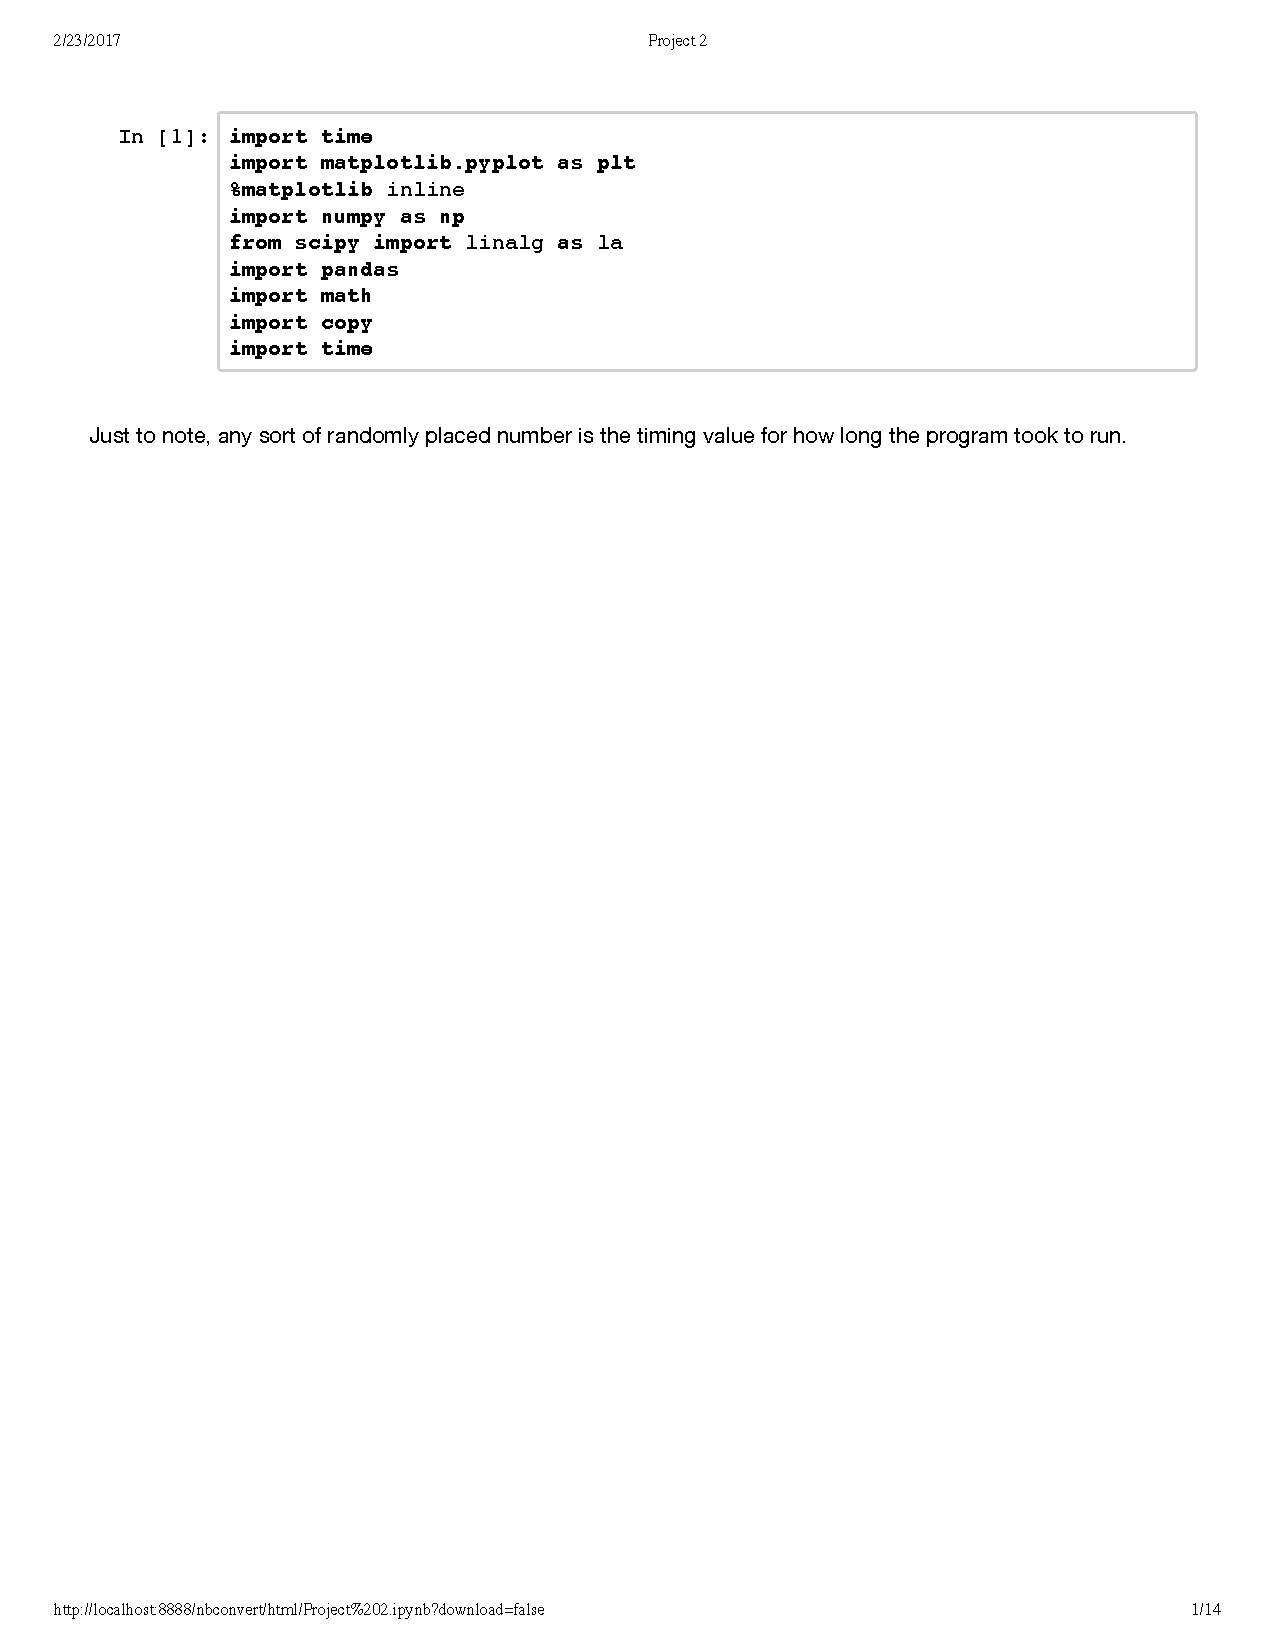
\includepdf[pages=-]{Project_2.pdf}

\end{document}

